\documentclass[journal,twoside,10pt]{IEEEtran}

% Packages
\usepackage{cite}
\usepackage[T1]{fontenc}
\usepackage{url}
\usepackage{amsmath,amssymb,amsfonts}
\usepackage{algorithmic}
\usepackage{graphicx}
\usepackage{textcomp}
\usepackage{xcolor}
\usepackage{listings}
\usepackage{afterpage}

% Custom section formatting for IEEEtran
\makeatletter
% Use Roman numerals for sections
\renewcommand\thesection{\Roman{section}}
% Format sections with Roman numerals and add period
\renewcommand\section{\@startsection{section}{1}{\z@}%
                       {-3.5ex \@plus -1ex \@minus -.2ex}%
                       {2.3ex \@plus.2ex}%
                       {\normalfont\Large\bfseries\Roman{section}.\quad}}
% Keep subsections unnumbered with no dot
\renewcommand\thesubsection{}
% Redefine subsection to avoid using any numbering
\renewcommand\subsection{\@startsection{subsection}{2}{\z@}%
                       {-3.25ex\@plus -1ex \@minus -.2ex}%
                       {1.5ex \@plus .2ex}%
                       {\normalfont\large\bfseries}}
% Empty section format to prevent automatic numbering
\renewcommand\@seccntformat[1]{}
\def\IEEEkeywordsname{Keywords}
\makeatother

% Configure listings package with enhanced JSON styling
\lstdefinestyle{mystyle}{
    backgroundcolor=\color{gray!10},
    commentstyle=\color{green!50!black},
    keywordstyle=\color{blue},
    stringstyle=\color{purple},
    basicstyle=\ttfamily\small,
    breakatwhitespace=false,
    breaklines=true,
    captionpos=b,
    keepspaces=true,
    numbers=none,
    numbersep=5pt,
    showspaces=false,
    showstringspaces=false,
    showtabs=false,
    tabsize=2
}

% Custom JSON styling
\lstdefinelanguage{JSON}{
    morestring=[b]",
    stringstyle=\color{purple},
    showstringspaces=false,
    keywords={false,true,null},
    keywordstyle=\color{orange},
    morekeywords={[2]"task_id","task","plan","actions","step","controlLabel","controlText","function","args","file_path"},
    keywordstyle={[2]\color{blue}},
    sensitive=false,
    comment=[l]{//},
    commentstyle=\color{green!50!black},
    morecomment=[s]{/*}{*/},
    literate=
        {:}{{{\color{black}{:}}}}{1}
        {,}{{{\color{black}{,}}}}{1}
        {\{}{{{\color{black}{\{}}}}{1}
        {\}}{{{\color{black}{\}}}}}{1}
        {[}{{{\color{black}{[}}}}{1}
        {]}{{{\color{black}{]}}}}{1}
}

\lstset{style=mystyle}

\begin{document}

\title{From Text to Action: The Evolution of AI Systems from Large Language Models to Multi-Agent Architectures}

\author{
    \begin{tabular}{p{0.23\textwidth}p{0.23\textwidth}p{0.23\textwidth}p{0.23\textwidth}}
    \small Adriana González Ugalde & \small Néstor J. Hernández Bautista & \small Carlos Alberto Parra Arredondo & \small Juan Carlos Romero Ramírez \\
    \small \textit{Tecnológico de Monterrey} & \small \textit{Tecnológico de Monterrey} & \small \textit{Tecnológico de Monterrey} & \small \textit{Tecnológico de Monterrey} \\
    \small A00194173@tec.mx & \small A00394821@tec.mx & \small A00534649@tec.mx & \small A00785001@tec.mx \\
    \end{tabular}
}

\maketitle

\begin{abstract}
    Large Language Models (LLMs) are evolving into systems capable of performing multiple productive tasks. 
    Early breakthroughs enabled these models to autonomously select and use external tools. 
    Subsequent research focused on transforming these models into Large Action Models (LAMs) tailored for action execution. 
    More recently, integrating LAMs within multi-agent systems (MASs) has emerged as a promising strategy for tackling complex, real-world tasks. 
    This survey synthesizes historical progress, contemporary research, and future directions in the field—from LLMs using tools to MASs that achieve collaborative, autonomous task execution.
\end{abstract}

\begin{IEEEkeywords}
    Large Language Models, Tool Augmentation, Large Action Models, Multi-Agent Systems, Autonomous Agents, Collaborative AI, Human-AI Productivity
\end{IEEEkeywords}

\section{Introduction}
We have observed that Large language models (LLMs) show remarkable capabilities in natural language understanding and generation. 
In early stages, LLMs were inherently limited to text-based outputs and struggled with tasks requiring real-world action. 
Recent work has demonstrated that LLMs can be extended to identify and call appropriate tools, effectively bridging the gap between language and action. 
This survey examines the progression from tool-using LLMs to specialized Large Action Models (LAMs), and ultimately to multi-agent systems that harness these capabilities for collaborative, productive task execution.
We would like to structure this examination as follows:
\begin{itemize}
    \item \textbf{How we got here:} A brief history of LLMs' transformation through tool usage.
    \item \textbf{Where we are now:} The emergence of LAMs and their integration into multi-agent frameworks.
    \item \textbf{Where we could go next:} Challenges faced by current systems and potential directions for future research.
\end{itemize}

\section{Literature Review}

\subsection{From Language Models to Tool-Using Agents}

In recent years, the transformer architecture has established strong foundations for AI advancement , enabling commercial LLM products that have transformed how society views and uses artificial intelligence. From a product engineering perspective, where user interface design is an important component in the chain of value, the chat interface has been widely embraced. This rapid adoption is no coincidence, our first interactions with LLMs occurred through interfaces that create the impression of conversing with another person, resulting in a natural experience that increase user adoption.

Initially, the value users derived from these interfaces was largely limited to text generation. As interactions became multimodal, the term "Generative AI" became popular to describe these systems. This term reflects both their architectural approach to generating outputs and their perceived intelligence and creativity, their ability to create new ideas, images, and sounds. This framing helps us understand phenomena like "hallucinations" and other characteristics of these AI systems.

In brief, contrary to science fiction's predictions, we have developed a form of artificial intelligence that excels more at creative tasks than logical ones. This observation sets the foundation for our literature review: while current AI shows immense potential, it still lacks the reliability needed for complex task execution.

In this research exercise, we identify a trend of evolution that expands around 3 years, i.e., \cite{schick2023toolformer, qin2023toolllm}. Researchers noticed the potential of the LLMs to be used for more than just text generation, as they displayed an interesting ability to understand and produce structured output, there was a possibility of integration with existing software artifacts already in place, such as APIs, SDKs, and any other programmable interface.

API's are one of the most natural places to start with.  Toolformer (Schick et al., 2023)~\cite{schick2023toolformer} represents a breakthrough in addressing LLM limitations through tool integration, enabling models to autonomously determine when external tools are needed, select appropriate ones, and incorporate their outputs into ongoing language generation. Its distinctive self-supervised learning methodology implemented a streamlined three-step process that samples potential API calls using in-context learning, executing these calls to obtain results, and filtering them based on perplexity reduction. This approach created a more adaptive system capable of determining which tools benefit specific contexts without extensive human annotation.

Expanding this line of research, ToolLLM (Qin et al., 2023)~\cite{qin2023toolllm} introduced a comprehensive framework for training models to effectively utilize external tools through API calls. It contributes with three key innovations: a systematic methodology for converting conventional dialogue datasets into tool-use examples through automated annotation; ToolBench, a diverse dataset spanning over 16,000 real-world scenarios across various domains; and a training approach enabling models to make effective API calls without human intervention. Performance evaluations demonstrate that tool-augmented models significantly outperform standard approaches, particularly in generating syntactically correct API calls, tool selection, and output integration.

These complementary innovations represents a first step in improving the reliability of AI systems for performing specific tasks by establishing a new paradigm where language models can handle tasks beyond linguistics to perform useful, real-world operations. By using its abilities for language understanding while gaining access to specialized functionality, tool-augmented systems offer a cost-effective approach to enhancing model capabilities without increasing model size, showing potential for transforming how AI assistants support human productivity across diverse domains.

\subsection{Large Action Models (LAMs)}
Tool-using LLMs introduced a paradigm shift in how we perceive AI systems' functionality. The breakthrough concept was simple yet powerful: "Now we have a system that can interact with our world", specifically within the context of modern digital productivity tools. Taking a step further in the evolution of  an LLM using tools, our research found the concept of "Large Action Models" which introduces a new action layer that positions AI systems at the same level of interaction as modern application layers. This advancement has produced systems capable of performing actions in dynamic environments. Although LAMs did not require significant architectural changes to LLMs, the name effectively captured the new direction of applied AI. We now proceed to describe this process.
To transform a general-purpose LLM into a specialized action execution system, a dedicated pipeline is required. Wang et al.~\cite{wang2025lam} detail this process comprehensively. Understanding this pipeline is important, not just for this paper, but because these methods can be broadly applied to similar objectives, deepening our understanding for future development. The process comprises several interconnected stages, which we will now explain:

\paragraph{Data Collection and Preparation}
As with most AI related work, everything starts with gathering and curating task-specific data. This initial phase follows a two-phase approach:

\begin{itemize}
    \item \textbf{Task-Plan Data Collection}: This involves collecting user requests and corresponding step-by-step plans. Sources include application documentation, WikiHow articles, and historical search queries. Each entry typically contains a task description and a detailed plan outlining the steps required to accomplish it.
    
    \item \textbf{Task-Action Data Collection}: This phase converts task-plan data into executable task-action data. Each plan step is transformed into concrete, actionable instructions that can be directly executed in the target environment. This process includes instantiation (adding specific operational details), execution validation, and evaluation to ensure correctness.
\end{itemize}

For example, a typical entry might look like:

\begin{lstlisting}[language=JSON]
{
  "task_id": "powerpoint_task_001",
  "task": "Create a slide based on draft.docx",
  "plan": [
    "1. Open the draft.docx and read the content.",
    "2. Create a new PowerPoint file.",
    "3. For page 1, add ..."
  ],
  "actions": [
    {
      "step": "open the document",
      "function": "open",
      "args": {"file_path": "draft.docx"}
    }
  ]
}
\end{lstlisting}

\paragraph{Transforming an LLM into a LAM, a Four-Phase Approach}

\begin{figure}[htbp]
    \centering
    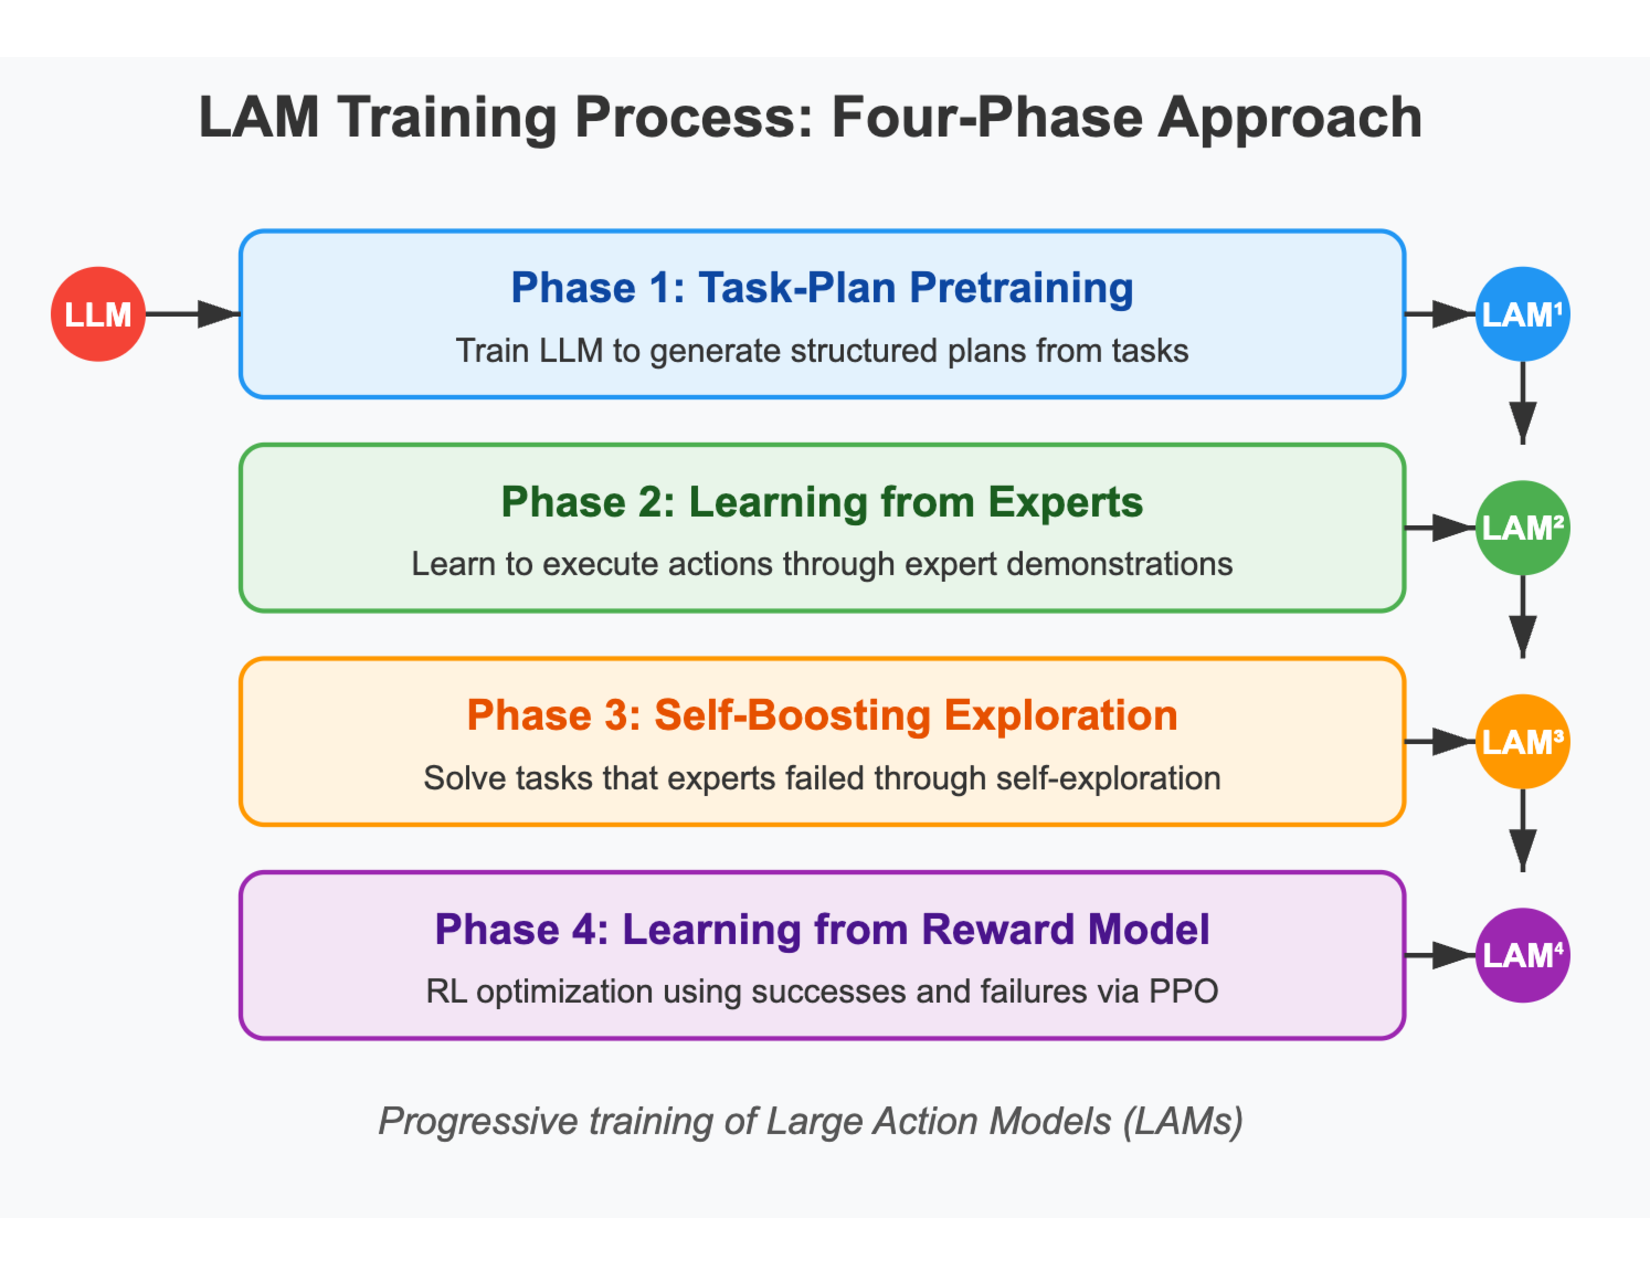
\includegraphics[width=0.5\textwidth]{traning_phases.pdf}
    \caption{Progressive four-phase training approach for transforming a general LLM into a specialized LAM.}
    \label{fig:lam-training}
\end{figure}

Wang et al.~\cite{wang2025lam} propose a systematic, four-phase training process that progressively builds capabilities from planning to action execution. As our LLM model progresses through these phases, it becomes a LAM:

\begin{enumerate}
    \item \textbf{Task-Plan Pretraining}: In this foundational phase, the model (LAM$^1$) learns to generate structured, step-by-step plans for completing tasks. Using supervised fine-tuning with task-plan pairs, the model develops the ability to break tasks into logical sequences. At this stage, the model can generate coherent plans but lacks execution capabilities.
    
    \item \textbf{Learning from Experts}: In the second phase, the model (LAM$^2$) learns to translate plans into concrete, executable actions through expert demonstrations. Training uses state-action pairs where each state includes the current UI environment and task context, and each action specifies which control to interact with and how. This phase grounds the model's reasoning in real application environments.
    
    \item \textbf{Self-Boosting Exploration}: In the third phase, the system learns to improve itself. LAM$^2$ attempts to solve tasks that were unsuccessful in previous stages. Using a ReAct mechanism \cite{yao2022react}, it interacts with the environment and explores alternative strategies for these challenging tasks. When successful, it generates new solutions. These solutions are then combined with the original expert examples to create an enhanced training dataset for LAM$^3$.
    
    \item \textbf{Learning from a Reward Model}: The final phase introduces reinforcement learning, enabling the model to learn from both successes and failures. First, a reward model is trained on both successful and failed trajectories, assigning positive values to successful steps and negative values to failures. Then, LAM$^4$ is fine-tuned using Proximal Policy Optimization (PPO) on previously failed trajectories, guided by the reward model's feedback. This approach enhances the model's decision-making abilities in complex scenarios.
\end{enumerate}

Each step in the training process builds on the one before it. This creates AI systems that get better and better at four key things: Planning out steps to solve problems, learning from expert examples, figuring things out on their own, getting better through trial and error.

\paragraph{Integration with Agents}
Once the training is complete, it is necessary to close the breach between strategy and execution. In few words, we have a very capable model to engage in planning to resolve tasks, but it's necessary to add interaction with the environment where it will operate. We introduce the concept of Agents—though their meaning and specific definition are still evolving—which, in the context of this paper, represent a layer of interaction between LAMs and the environment. LAMs must be integrated into an agent framework to interact with real-world environments. To make LAMs work in the real world, they need four main parts working together:

\begin{enumerate}
    \item A way to see and understand what's happening in their environment, usually through special software interfaces (UI Automation APIs)
    \item A system that turns the model's decisions into actual actions in the environment
    \item A memory system that keeps track of what actions were taken and what plans were made, helping the system stay organized and consistent
    \item A feedback system that watches how the environment responds to actions, helping the system learn and adjust to changes
\end{enumerate}

Put simply, the LAM functions as the brain while the Agents serve as the body, complete with hands that can manipulate tools and execute plans.

\paragraph{Evaluation}
Evaluation is a critical component of any DL/ML system, serving as the feedback loop for system improvement. While Wang and colleagues~\cite{wang2025lam} established clear testing methodologies for comparing different versions and ensuring proper functionality across various situations, the current evaluation scope remains limited to a 435-task benchmark focused on Microsoft Word tasks. Nevertheless, their comprehensive development pipeline demonstrates LAMs' ability to translate user intentions into meaningful actions within specific operational contexts, representing a utility advancement over traditional text-generation models by enabling the execution of complex, multi-step tasks in real-world environments—though more extensive testing across diverse domains is still needed.

LAMs enable a wide range of applications previously challenging for traditional LLMs, including:

\begin{itemize}
    \item Autonomous interaction with Operating Systems through CLI interfaces.
    \item Control of User Interfaces which are present in most of the software applications.
    \item The potential for complex task automation in specialized domains.
    \item Multi-step problem-solving that requires environmental awareness
\end{itemize}

LAMs thus represent a paradigm shift—from language generation to action execution—allowing AI systems to automate complex processes with minimal human intervention, substantially expanding their practical utility across numerous domains.

\subsection{Multi-Agent Systems}

\begin{figure}[htbp]
    \centering
    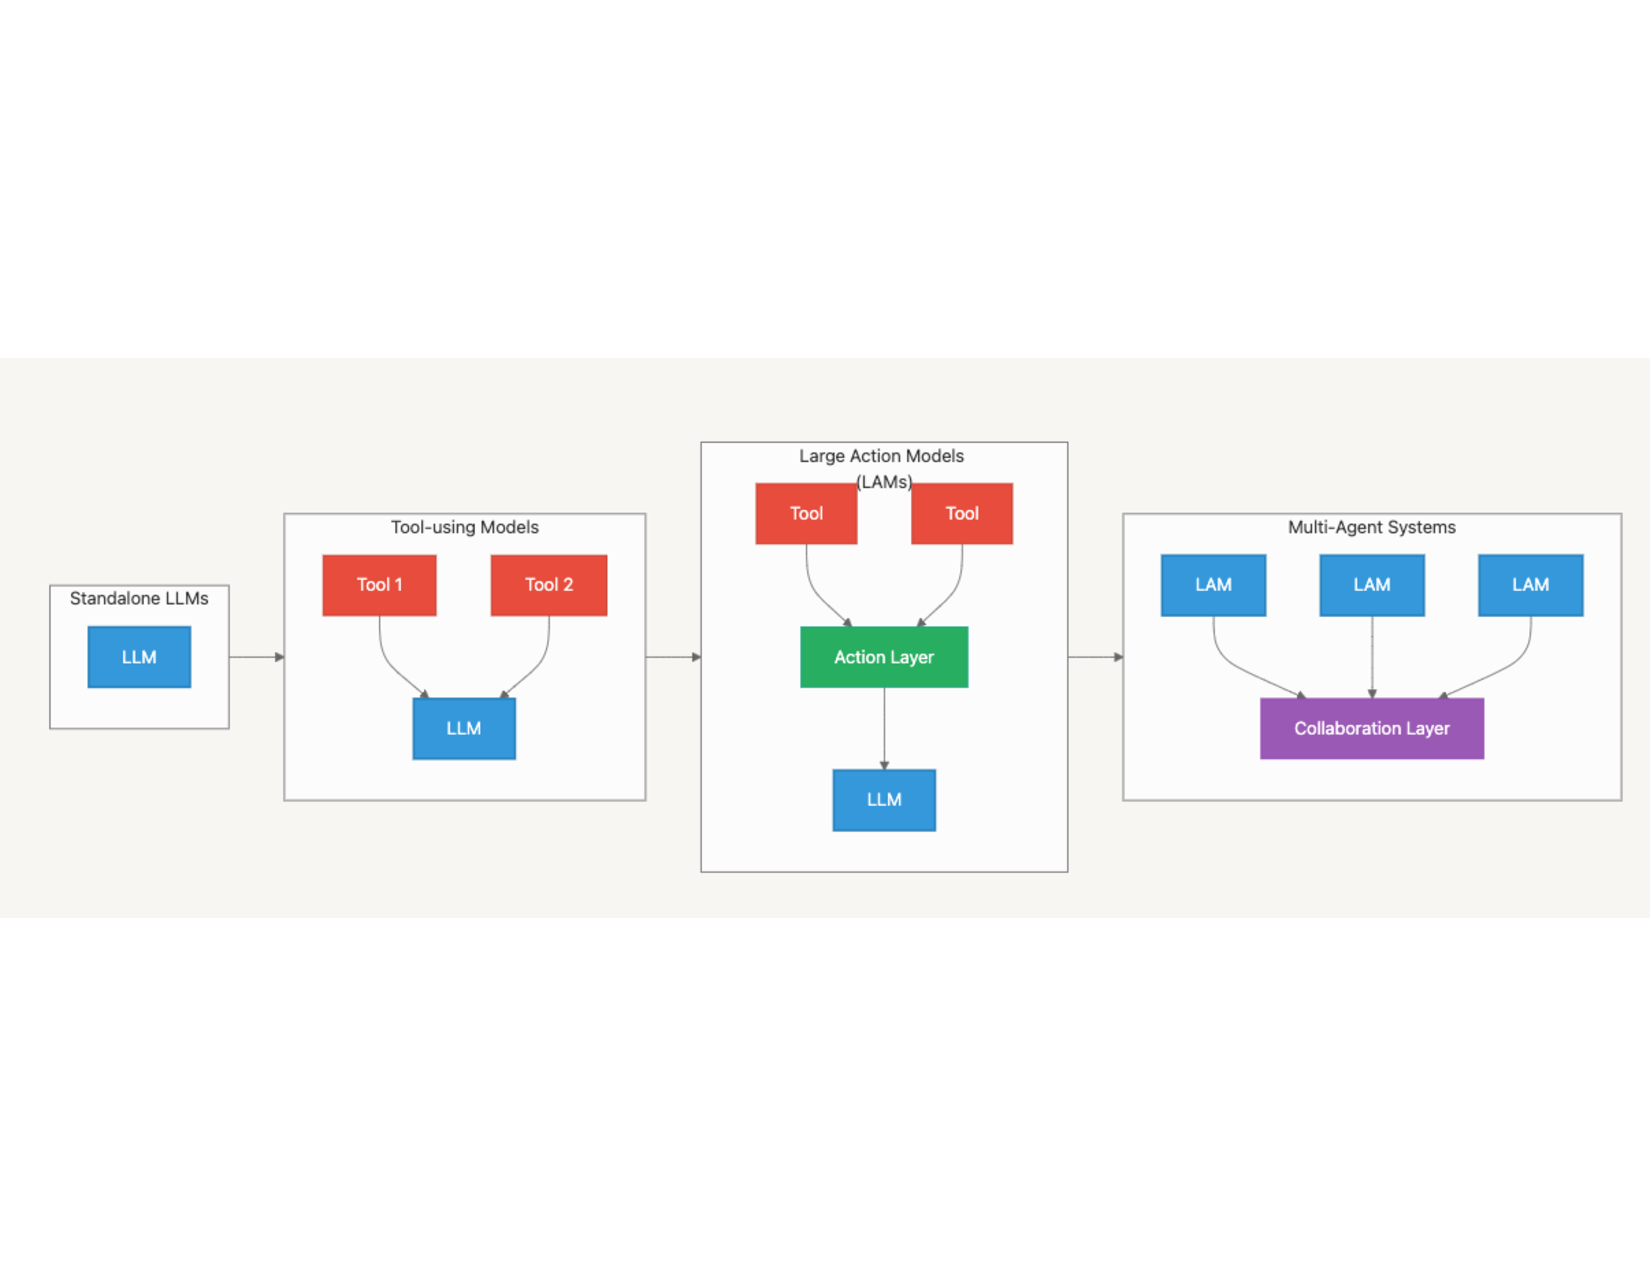
\includegraphics[width=0.5\textwidth, trim=0 150pt 0 150pt, clip]{lams_diagram.pdf}
    \caption{Evolution of AI systems from standalone LLMs to multi-agent systems.}
    \label{fig:lam-evolution}
\end{figure}

Let's take a brief pause and look at how our initial systems have evolved over time. First, we had LLM models that learned to use simple tools. Next, with more training, these models became better at making plans and developing strategies. Finally, when we combined these models with an agentic layer, they got much better at doing real-world tasks. We identify a collaborative approach that fundamentally transforms how AI operates by shifting from isolated models toward interconnected systems that can distribute complex problems. We now introduce the concept of Multi-Agent Systems. If the challenge with LAMs was to design specific training to specialize our LLM, now the challenge for multi-agent systems is to establish robust methods for a collaboration layer, which should enable them to communicate, coordinate, and collectively tackle complex, multi-step challenges. The following section will try to bring an overview of this important collaboration layer component.

According to \cite{tran2025multiagent}, the collaboration mechanisms in these systems can take various forms: Cooperation, competition and a hybrid approach named Coopetition. In cooperative scenarios, agents align their individual objectives with shared goals, often specializing in complementary roles to enhance efficiency. This approach has proven successful in applications ranging from question answering to collaborative programming, where different agents may handle research, planning, execution, and evaluation tasks. By contrast, competitive collaboration occurs when agents operate with potentially conflicting objectives, which can drive innovation and robustness through evolutionary pressure. Such competition-based approaches have shown benefits in debate frameworks and strategic gaming environments, where contradictory perspectives often yield more nuanced and comprehensive solutions. A hybrid approach, coopetition, enables agents to collaborate on certain tasks while competing on others, facilitating negotiation and compromise in complex, multi-objective problems.

Communication is another important component as it defines the information flow between agents. In centralized architectures, communication follows a star structure  where interactions flow through a central coordinator agent that manages task allocation and synthesizes results. On the other hand decentralized structures enable peer-to-peer interactions without centralized control, offering greater resilience against single points of failure, although there is a downside, as more sophisticated coordination mechanisms are required. The communication system could also have a hierarchical arrangement by creating layered structures with defined authority levels, this balance control and flexibility across different tiers of agents with varying specializations.

In our research, we noticed significant enthusiasm for agentic systems across various tech communities. Through examining relevant papers, we identified that successful implementation and adoption of these systems depends heavily on addressing key challenges outlined in this paper. For example, to make these communication structures work effectively, a common protocol must be defined. This protocol should accommodate three essential factors that govern AI agent collaboration:

\begin{enumerate}
    \item It should be rule-based: Having clear, predefined guidelines that specify how agents interact with each other
    \item It should allow for role-based systems: Assigning different jobs to different agents based on their specific capabilities
    \item Flexible systems: Enabling behavior adjustment based on changing situations and uncertainties
\end{enumerate}

These systems ensure AI agents collaborate in an organized and effective manner. We expect to see more solutions addressing this key challenge in the coming year. It's worth noting Anthropic's Model Context Protocol (MCP) which, despite lacking academic publication, demonstrates promising adoption and usability in addressing the previously discussed challenges.
\subsection{Applications and Use Cases}
Let's pause to examine some key characteristics of the systems reviewed in this paper. While showing significant advancement over time, these systems consistently employ a three-component architecture for information processing and decision-making:

\begin{enumerate}
    \item A state encoder that processes structured input
    \item A policy network that generates appropriate actions
    \item A value network that evaluates the potential outcome of those actions
\end{enumerate}

Through this lens, we would briefly like to present some applications and use cases across several domains that highlight the usage of these components.
In strategic gaming, DeepMind's AlphaGo achieved a historic milestone as the first AI system to defeat a human champion at Go, combining advanced neural networks with Monte Carlo Tree Search (MCTS) to evaluate board positions and optimize complex strategies \cite{silver2016mastering}. Extending these capabilities, OpenAI Five mastered the multiplayer game Dota 2 through self-play and Proximal Policy Optimization, demonstrating how these systems can effectively handle dynamic environments with multiple interacting agents \cite{openai2019dota}.

More recently, Salesforce has brought these capabilities into the commercial sphere with its xLAM series—a family of Large Action Models designed for practical applications \cite{zhang2024xlam}. These models, available in various sizes and configurations, demonstrate exceptional proficiency in executing real-world tasks through effective tool utilization and interactive operations, representing a significant step toward consumer-oriented implementations of this technology.
\section{Future Directions} 

Having reviewed the fundamental components of multi-agent systems, we can explore another branch of evolution in AI architecture: Large Multimodal Action Models. 
While LAMs excel at processing structured, state-based inputs to produce optimal actions, these models would represent a significant advancement by incorporating diverse multimodal inputs—including visual data, natural language, and sensor information. This enhanced capability allows them to operate effectively in unstructured, complex environments, making them particularly suitable for robotics, autonomous driving, sophisticated digital assistants, and human-robot collaboration scenarios. 
As these models continue to expand into various domains, new challenges emerge that require focused research in physical and multi domain interactions. We will now briefly expose some research initiatives that have established promising foundations in this concept, demonstrating how the integration of Large Multimodal Action Models with multi-agent systems could dramatically expand AI capabilities.

\begin{itemize}
    \item \textbf{RT-2} by Google DeepMind \cite{brohan2023rt2}, functions as a Vision-Language-Action transformer, using a vision transformer to encode visual input, a language model to process textual commands, and an action decoder that generates precise motor commands through cross-attention mechanisms between visual and language embeddings.
    
    \item \textbf{Gato}, also developed by DeepMind \cite{reed2022generalist}, represents a unified approach through a single transformer architecture that processes multiple input modalities (text, images, and state information) into a common embedding space before generating appropriate action predictions across diverse tasks.
    
    \item \textbf{PaLM-E} from Google, \cite{driess2023palme}, combines a foundation language model (PaLM) with specialized vision encoders and embodied control modules, enabling joint processing of natural language instructions and visual inputs to produce coordinated robotic actions via a transformer-based decoder.
\end{itemize}

As multi-agent systems continue to evolve, we anticipate that these models will generate widespread adoption across diverse applications, with commercial deployment accelerating rapidly in the years ahead. This expansion, however, presents significant challenges in computational efficiency, privacy safeguards and security measures.

\section{Conclusion}

This work has examined the progression from large language models to multi-agent systems, representing a significant advancement in artificial intelligence capabilities. In our analysis we have studied how AI has expanded its practical applications across various domains, enabling sophisticated automation of tasks that traditionally required human oversight. Although significant progress has been made, key challenges remain in the development of reliable coordination mechanisms, standardized communication protocols, effective error management, and comprehensive evaluation frameworks. 
Future research initiatives should prioritize the development of robust frameworks that enhance agent collaboration, establish standardized communication protocols, and implement specialized performance metrics for multi-agent interactions.It was interesting to notice that many of the methods used to develop these systems have existed for quite some time. We observe this pattern in the studied transformation of LLMs into LAMs, and perhaps more recently and notably in the use of traditional methodologies like reinforcement learning, which aids in the development and optimization of the Deepseek, \cite{liu2024deepseekv3} model.
Looking ahead, we expect these systems to grow from experimental projects into real business solutions that can handle complex tasks together, both in computer systems and in the real world. This advancement in technology will not only improve what we can already do but could completely change how humans and AI work together across many different industries.


\bibliographystyle{IEEEtran}
\bibliography{references}
 
\end{document}